\section{Validation}

To check to model from the paper, the following parameters are used:

\begin{figure}[H]
	\centering
	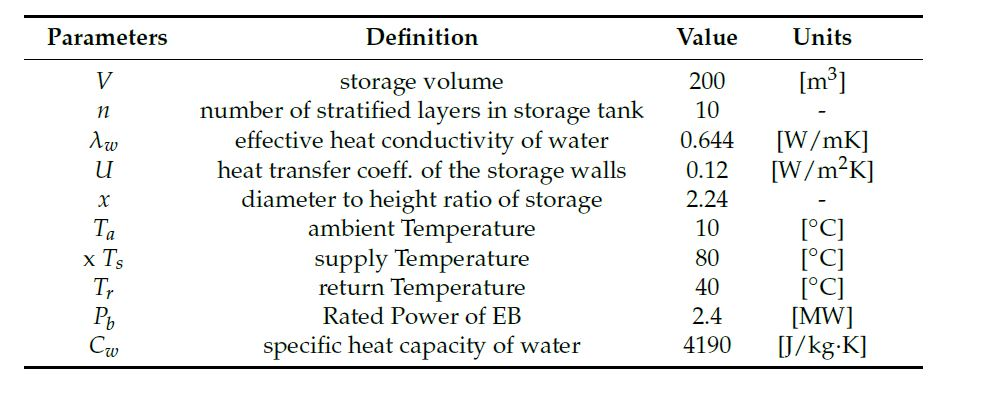
\includegraphics[width=0.8\columnwidth]{Pictures/parameters_paper.JPG}
	\caption[Short title]{Buffer vessel parameters}
\end{figure}

This results in the following graph:

\begin{figure}[H]%
	\centering
	\subfloat[\centering paper results]{{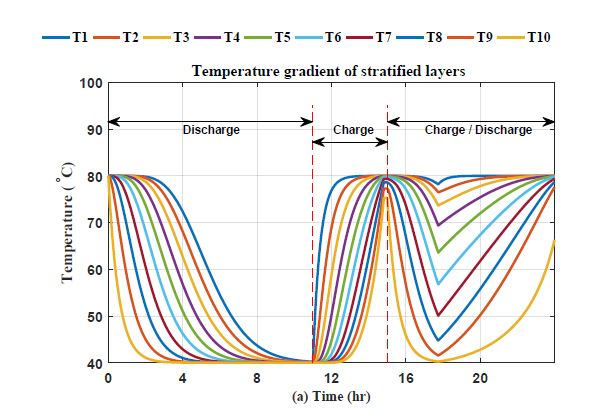
\includegraphics[width=0.8\columnwidth]{Pictures/paper_results.jpg} }}%
	\qquad
	\subfloat[\centering Python results]{{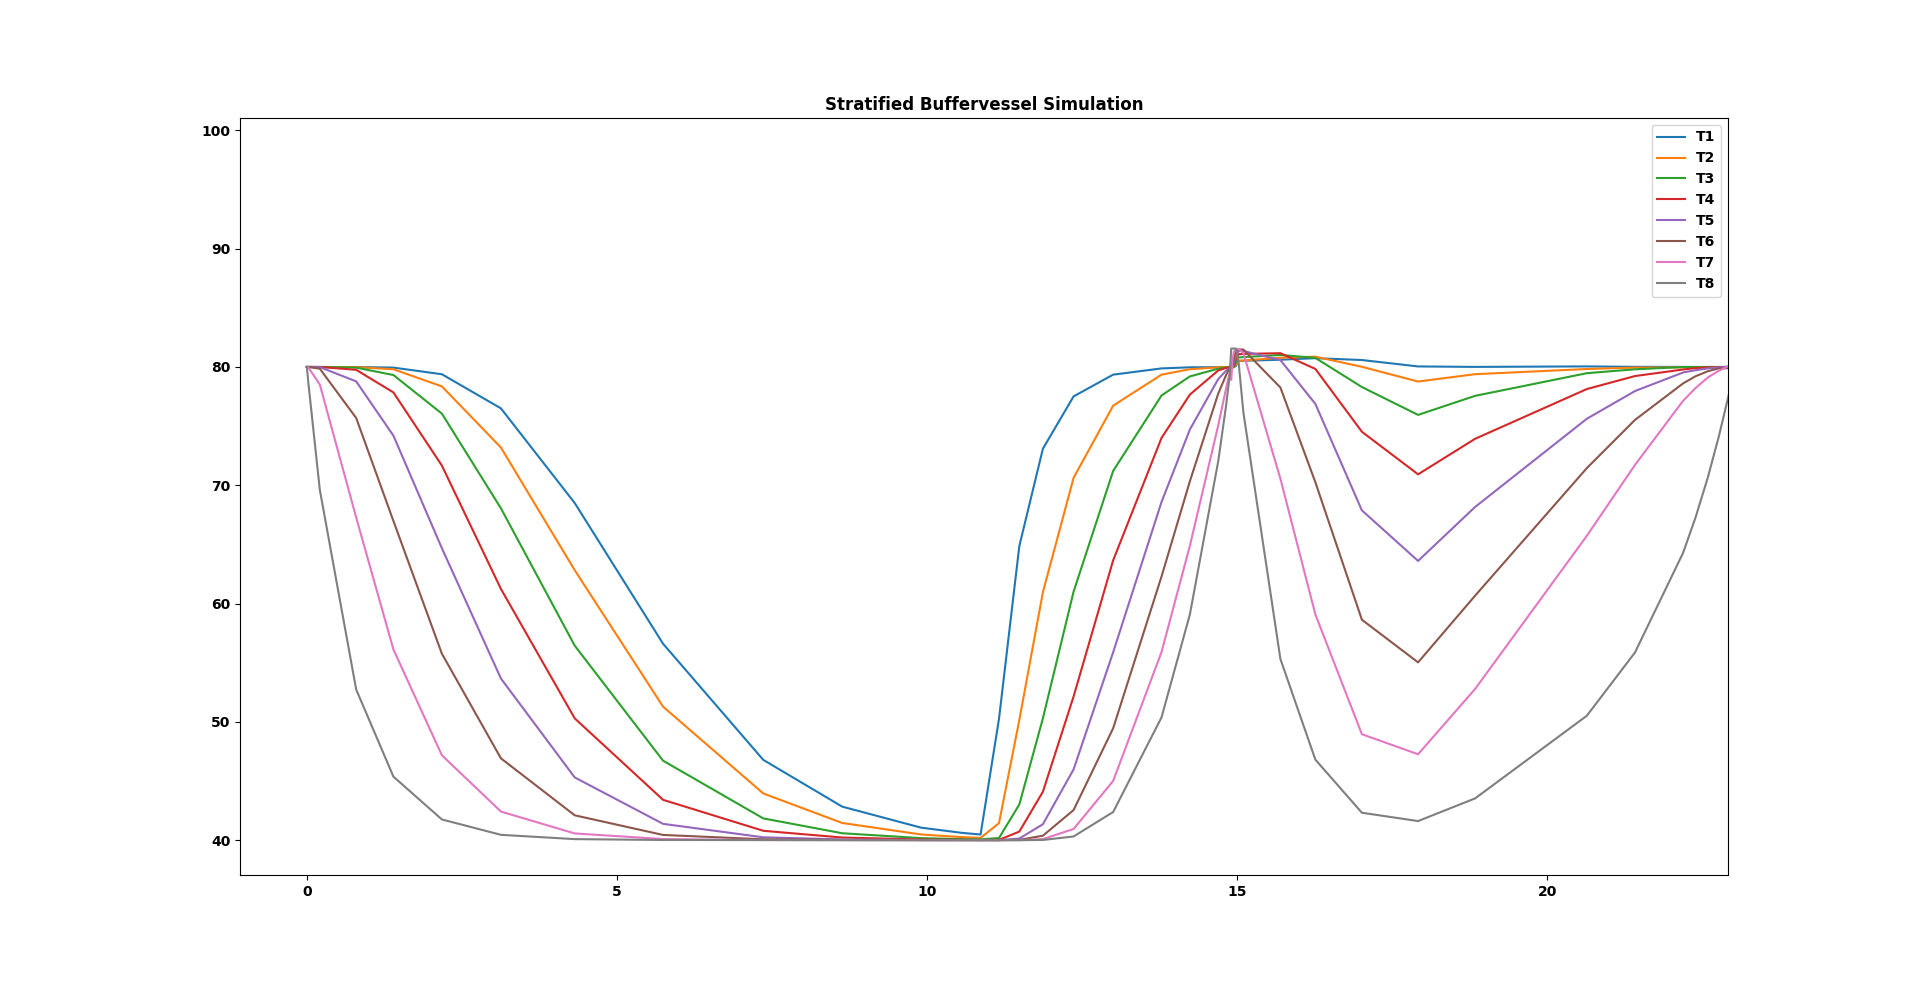
\includegraphics[width=0.8\columnwidth]{Pictures/Python_validation_graph_buffervessel.png} }}%
	\caption{Comparison between paper and python model}%
	\label{fig:Comparison}%
\end{figure}